\section{Дизайн библиотеки Roren}
\label{sec:design}

Дизайн библиотеки Roren построен аналогично open-source инструменту Apache Beam \cite{beam}.

Apache Beam предлагает универсальный API для создания сложных pipeline-ов обработки данных, которые можно запускать на различных движках. В случае Roren движки называют executor-ами. Основные принципы этого уровня основаны на модели Beam (ранее известной как модель Dataflow \cite{dataflow}) и реализованы в различной степени в каждом из executor-ов Roren.

Такой дизайн позволяет разработчикам проектировать масштабируемые приложения для обработки данных, которые могут адаптироваться к разным технологическим платформам и инфраструктурам без необходимости изменения кода. Использование Roren упрощает интеграцию с различными источниками данных и позволяет эффективно управлять потоками данных и их обработкой.

\newpage
\subsection{Interface graph}

Библиотека Roren включает в себя несколько абстракций, которые упрощают процесс обработки данных в условиях больших распределенных систем. Эти абстракции применимы как к batch, так и к streaming источникам данных. При создании pipeline-а есть возможность структурировать задачи обработки данных, используя абстракции преобразований данных и результатов их применений - transform-ов и collection-ов соответственно.

Pipeline описывает всю задачу обработки данных от начала до конца. Он включает в себя чтение входных данных, их преобразование и запись выходных таблиц. При его создании есть возможность указать параметры выполнения, специфичные для конкретного паттерна выполнения: настройки streaming или MapReduce инфраструктуры.

Collection представляет собой распределенный набор данных, с которым работает pipeline. Набор данных может быть ограниченным, то есть происходить из фиксированного источника, как файл, или неограниченным, то есть поступать из постоянно обновляющегося streaming источника. Типичный pipeline создает начальный collection, читая данные из внешнего источника данных. Далее, коллекции служат входными и выходными данными для каждого преобразования в pipeline.

Transform представляет операцию обработки данных. Каждый transform принимает один или несколько объектов collection в качестве входных данных, выполняет функцию обработки, которую пользователь предоставляет, над элементами этой коллекции данных, а затем производит ноль (в случае стока графа - записи во внешнее хранилище) или более выходных объектов collection.

Roren включает множество I/O преобразований - библиотечных transforms, которые читают или записывают данные в различные внешние системы хранения данных. Чтения и записи таблиц в случае MapReduce или топиков брокеров сообщений осуществляются через общие интерфейсы IRawRead и IRawWrite.

Трансформации могут изменять, фильтровать, группировать, анализировать или иным образом обрабатывать элементы collection-а. Преобразование создает новую выходную коллекцию данных, не модифицируя входную коллекцию. Типичный pipeline применяет последующие трансформации к каждой новой выходной collection по очереди, пока обработка не будет завершена. Однако стоит отметить, что пайплайн не обязательно должен быть одной прямой линией трансформаций, применяемых одна за другой. Можно рассматривать коллекции как переменные, а преобразования как функции, применяемые к этим переменным, что позволяет создать сложный граф обработки.

После того, как в коде описаны все transform-ы, pipeline запускается с использованием назначенного executor-а (рис~\ref{fig:pipeline}).

\begin{figure}[h]
    \centering
    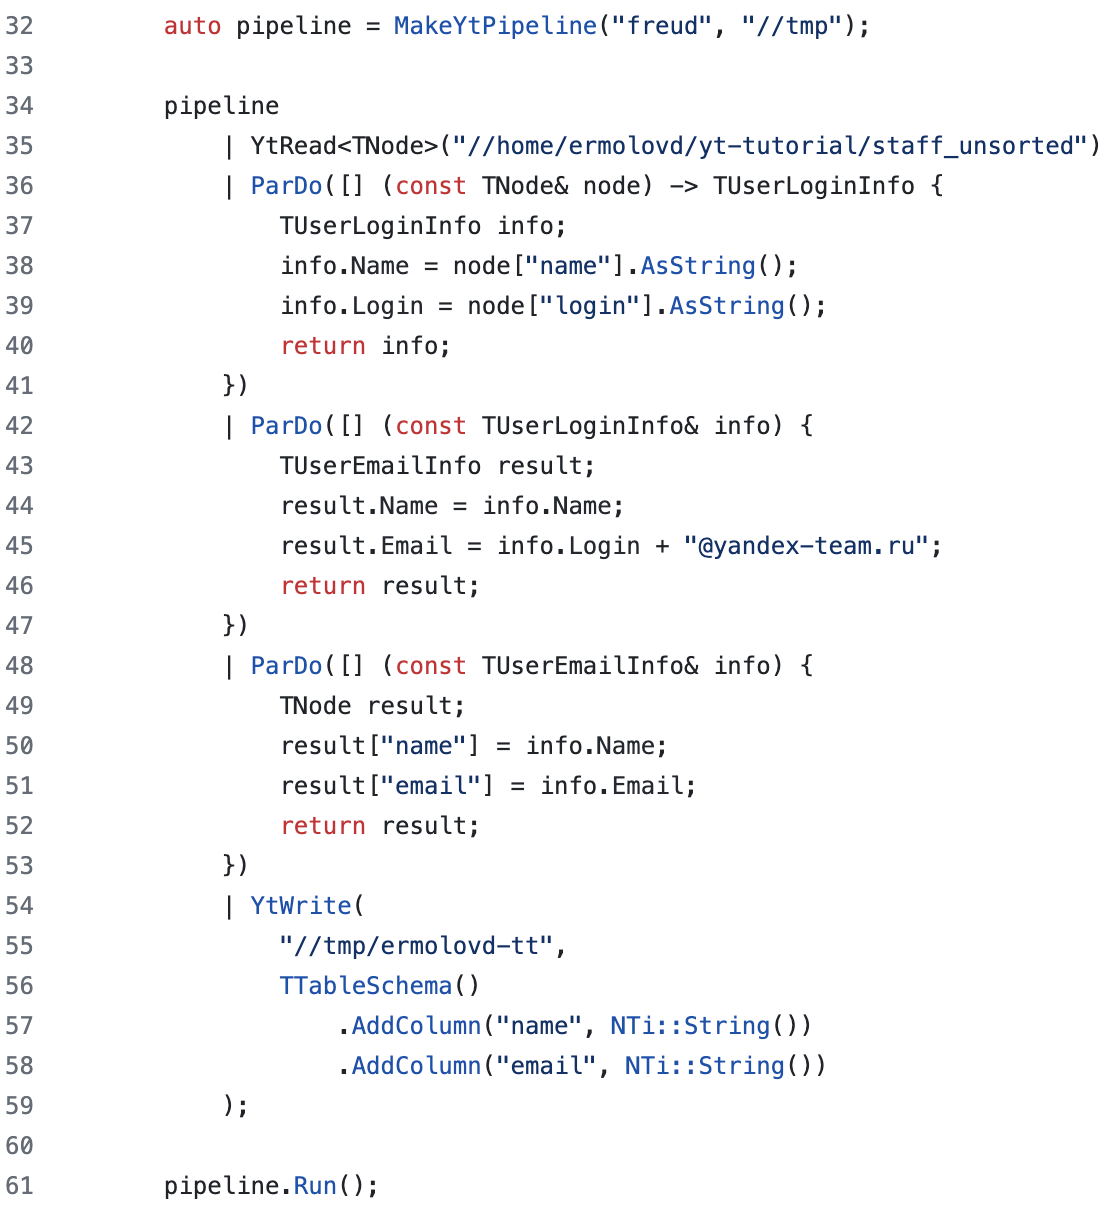
\includegraphics[width=\textwidth]{img/pipeline.png}
    \caption{Типичный pipeline с YT executor-ом}
    \label{fig:pipeline}
\end{figure}

\newpage
\subsection{Понятие executor-а}

Executor - это движок, отвечающий за то, каким именно образом данные поступают и обрабатываются графом transform-ов.

В простейшем случае streaming процессинга пользователь указывает входные топики брокера логов или очереди сообщений, ожидая, что данные относительно небольшими порциями будут вычитаны из источников, к ним применяются transform-ы и они будут записаны в выходные топики, очереди или таблицы.

В случае batch процессинга после указания входных и выходных таблиц с помощью примитивов API pipeline-а ожидается запуск некоторого количества операций, а как следствие Map/Reduce job-ов на кластере. Вместе эти операции будут эквивалентны применению к входным данным преобразований, указанных пользователем.

На этом этапе можно задуматься, что ParDo соответствует Map операции запущенной на кластере, а GroupByKey - Reduce.

\newpage
\subsection{YT executor}

Далее мы рассмотрим специфику запуска именно на YT Map/Reduce кластере.

Api YT имеет возможность создания операций с многими входами, многими выходами. Причем зачастую, есть возможность писать выходные таблицы с промежуточных стадий составных операций.

Если рассмотреть некоторый подграф, состоящий целиком из ParDo, то теоретически ничто не мешает запустить его как одну Map операцию, которая внутри себя сохраняет структуру вызова пользовательских функций из ParDo. Наличие возможности указать многие входы и выходы операции позволяет запускать подграфы с несколькими истоками и стоками.

В свою очередь, GroupByKey в общем случае может быть представлен в виде MapReduce операции. Это объясняется тем, что перед функцией группировки будут вызвано какое-то количество ParDo преобразующих входные данные из YSON \cite{yson} формата во внутреннее представление пары ключ-значение.

Существует важное замечание, что MapReduce - это операция Map, решардирование с помощью хэширования и запуск Reduce. Такого рода операция эффективнее Map, сортировки данных и Reduce.

I/O общение с таблицами кластера осуществляется через реализацию RawRead и RawWrite - YtRead и YtWrite. C помощью YtRead можно чтения таблиц в YSON или Protobuf \cite{protobuf} форматах. YtWrite имеет возможность указания схемы, в том числе сортированной, для записи выходных значений. Так как рассматриваемая в данной работе реализация является proof-of-concept, мы опускаем реализации I/O в формате Protobuf и сортированных данных.

